\chapter{Risorse}
\newpage

\section{Introduzione}
Un sistema di elaborazione è composto da un insieme di risorse da assegnare ai processi presenti.
I processi competono nell'accesso alle risorse.

\textit{Esempi di risorse: memoria, stampanti, processore, dischi
interfaccia di rete, descrittori di processo...}

\subsection{Classi di risorse}
Le risorse possono essere suddivise in classi, le risorse appartenenti alla stessa classe sono equivalenti.
\textit{Esempi: byte della memoria, stampanti dello stesso tipo, etc.}

Le risorse di una classe vengono dette \textbf{istanze della classe}, il numero di risorse in una classe viene detto \textbf{molteplicità} del tipo di risorsa.

Un processo non può richiedere una specifica risorsa, ma solo una risorsa di una specifica classe. Una richiesta per una classe di risorse può essere soddisfatta da qualsiasi istanza di quel tipo.

\subsubsection{Assegnazione delle risorse}
\paragraph{Risorse ad assegnazione statica}
Avviene al momento della creazione del processo e rimane valida fino alla terminazione.

\textit{Esempi: descrittori di processi, aree di memoria (in alcuni casi)}

\paragraph{Risorse ad assegnazione dinamica}
I processi richiedono le risorse durante la loro esistenza, le utilizzano una volta ottenute e le rilasciano quando non più necessarie.

\textit{Esempi: periferiche di I/O, aree di memoria (in alcuni casi)}

\subsubsection{Tipi di richieste}
\paragraph{Richiesta singola}
Si riferisce a una singola risorsa di una classe definita, è il caso normale.

\paragraph{Richiesta multipla}
Si riferisce a una o più classi, e per ogni classe, ad una o più risorse, deve essere soddisfatta integralmente.

\paragraph{Richiesta bloccante}
Il processo richiedente si sospende se non ottiene immediatamente
l'assegnazione, la richiesta rimane pendente e viene riconsiderata dalla funzione di gestione ad ogni rilascio.

\paragraph{Richiesta non bloccante}
La mancata assegnazione viene notificata al processo richiedente, senza provocare la sospensione.

\subsubsection{Tipi di risorse}

\paragraph{Risorse seriali (o con accesso mutuamente esclusivo)}
Una singola risorsa non può essere assegnata a più processi contemporaneamente.

\textit{Esempi: i processori, le sezioni critiche, le stampanti}

\paragraph{Risorse non seriali}

\textit{Esempio: file di sola lettura}


\paragraph{Definizione:} Una risorsa si dice prerilasciabile se la funzione di gestione può sottrarla ad un processo prima che questo l'abbia effettivamente rilasciata.

\paragraph{Meccanismo di gestione:} Il processo che subisce il prerilascio deve sospendersi, la risorsa prerilasciata sarà successivamente restituita al processo.

Una risorsa è prerilasciabile: se il suo stato non si modifica durante l'utilizzo oppure il suo stato può essere facilmente salvato e ripristinato.

\textit{Esempi: processore, blocchi o partizioni di memoria
(nel caso di assegnazione dinamica)}

\subsection{Risorse non prerilasciabili}

\paragraph{Definizione:} La funzione di gestione non può sottrarle al processo al quale sono assegnate, sono non prerilasciabili le risorse il cui stato non può essere salvato e ripristinato.

\textit{Esempi: stampanti, classi di sezioni critiche, partizioni di memoria (nel caso di gestione statica)}

\section{Deadlock}
Come abbiamo visto i deadlock impediscono ai processi di terminare correttamente, inoltre le risorse bloccate in deadlock non possono essere utilizzati da altri processi.

Vedremo ora le condizioni che necessarie affinché un deadlock si presenti e le tecniche che possono essere utilizzate per gestire  questo problema.

\subsection{Condizioni per avere deadlock}
\begin{itemize}
    \item \textbf{Mutua esclusione:} le risorse coinvolte devono essere seriali
    \item \textbf{Assenza di prerilascio:} le risorse coinvolte non possono essere prerilasciate, ovvero devono essere rilasciate volontariamente dai processi che le controllano
    \item \textbf{Richieste bloccanti (detta anche "hold and wait"):} le richieste devono essere bloccanti, e un processo che ha già ottenuto risorse può chiederne ancora
    \item \textbf{Attesa circolare:} esiste una sequenza di processi $P_0$, $P_1$ , ..., $P _n$, tali per cui $P_0$ attende una risorsa controllata da $P_1$ e $P_1$ attende una risorsa controllata da $P_2$, ..., e $P_n$ attende una risorsa controllata da $P_0$.
\end{itemize}


L'insieme di queste condizioni è necessario e sufficiente. 
Devono valere tutte contemporaneamente affinché un deadlock si presenti nel sistema.

\subsection{Grafo di Holt}

\paragraph{Caratteristiche:} 
\begin{itemize}
    \item è un grafo diretto: gli archi hanno una direzione.
    \item è un grafo bipartito: i nodi sono suddivisi in due sottoinsiemi e non esistono archi che collegano nodi dello stesso sottoinsieme. I sottoinsiemi sono risorse e processi.
    \item gli archi risorsa → processo indicano che la risorsa è assegnata al processo.
    \item gli archi processo → risorsa indicano che il processo ha richiesto la risorsa.
\end{itemize}

\begin{figure}[h]
    \centering
    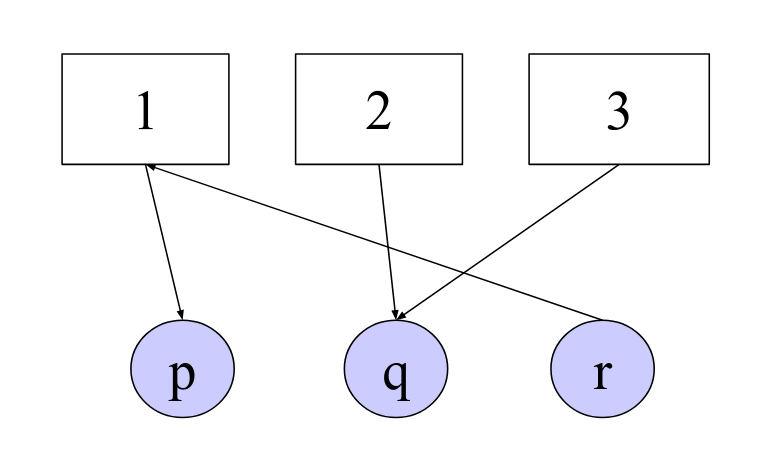
\includegraphics[width=0.4\linewidth]{Images/Screenshot 2024-12-30 at 18-00-42 so-04-risorse - so-04-risorse.pdf.png}
\end{figure}

\subsubsection{Grafo di Holt generale}
Nel caso di classi contenenti più istanze di una risorsa, l'insieme delle risorse è partizionato in classi e gli archi di richiesta sono diretti alla classe e non alla singola risorsa.

\paragraph{Rappresentazione:} i processi sono rappresentati da cerchi, le classi sono rappresentati come contenitori rettangolari
e le risorse come punti all'interno delle classi.

\textit{Nota: non si rappresentano grafi di Holt con archi relativi a richieste che possono essere soddisfatte, se esiste almeno un'istanza libera della risorsa richiesta, la risorsa viene
assegnata.}

\begin{figure} [h]
    \centering
    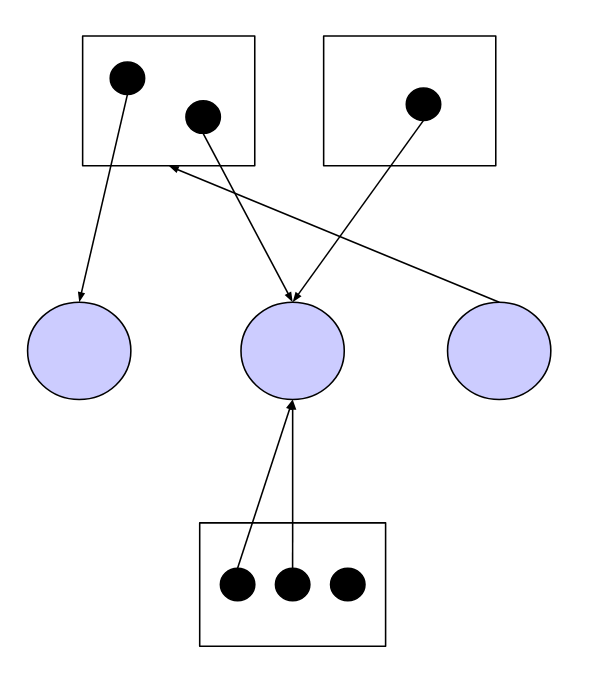
\includegraphics[width=0.2\linewidth]{Images/Screenshot 2024-12-30 at 18-04-17 so-04-risorse - so-04-risorse.pdf.png}
\end{figure}

Alcuni autori preferiscono indicare numericamente:
Sugli archi la molteplicità della richiesta
(archi processo → classe) e la molteplicità dell'assegnazione
(archi classe → processo).
All'interno delle classi il numero di risorse non ancora
assegnate.


\section{Metodi di gestione dei deadlock}

\begin{itemize}
    \item \textbf{Deadlock detection and recovery:} permettere al sistema di entrare in stati di deadlock; utilizzare un algoritmo per rilevare questo stato ed eventualmente eseguire un'azione di recovery.
    \item \textbf{Deadlock prevention / avoidance:} impedire al sistema di entrare in uno stato di deadlock
    \item \textbf{Ostrich algorithm:} ignorare il problema del tutto.
\end{itemize}

\subsection{Deadlock detection}
\paragraph{Descrizione} mantenere aggiornato il grafo di Holt, registrando su di esso tutte le assegnazioni e le richieste di risorse. Utilizzare il grafo di Holt al fine di riconoscere gli stati di deadlock.

\paragraph{Problema:} come riconoscere uno stato di deadlock?

\subsubsection{Caso 1 - Una sola risorsa per classe}

\paragraph{Teorema:} se le risorse sono ad accesso mutualmente esclusivo, seriali e non prerilasciabili, lo stato è di deadlock se e solo se il grafo di Holt contiene un ciclo.

\paragraph{Dimostrazione:} si utilizza una variante del grafo di Holt, detto grafo Wait-For, si ottiene un grafo wait-for eliminando i nodi di tipo risorsa e collassando gli archi appropriati, il grafo di Holt contiene un ciclo se e solo se il grafo Wait-for contiene un ciclo.
Se il grafo Wait-for contiene un ciclo, abbiamo attesa circolare

\begin{figure}[h]
    \centering
    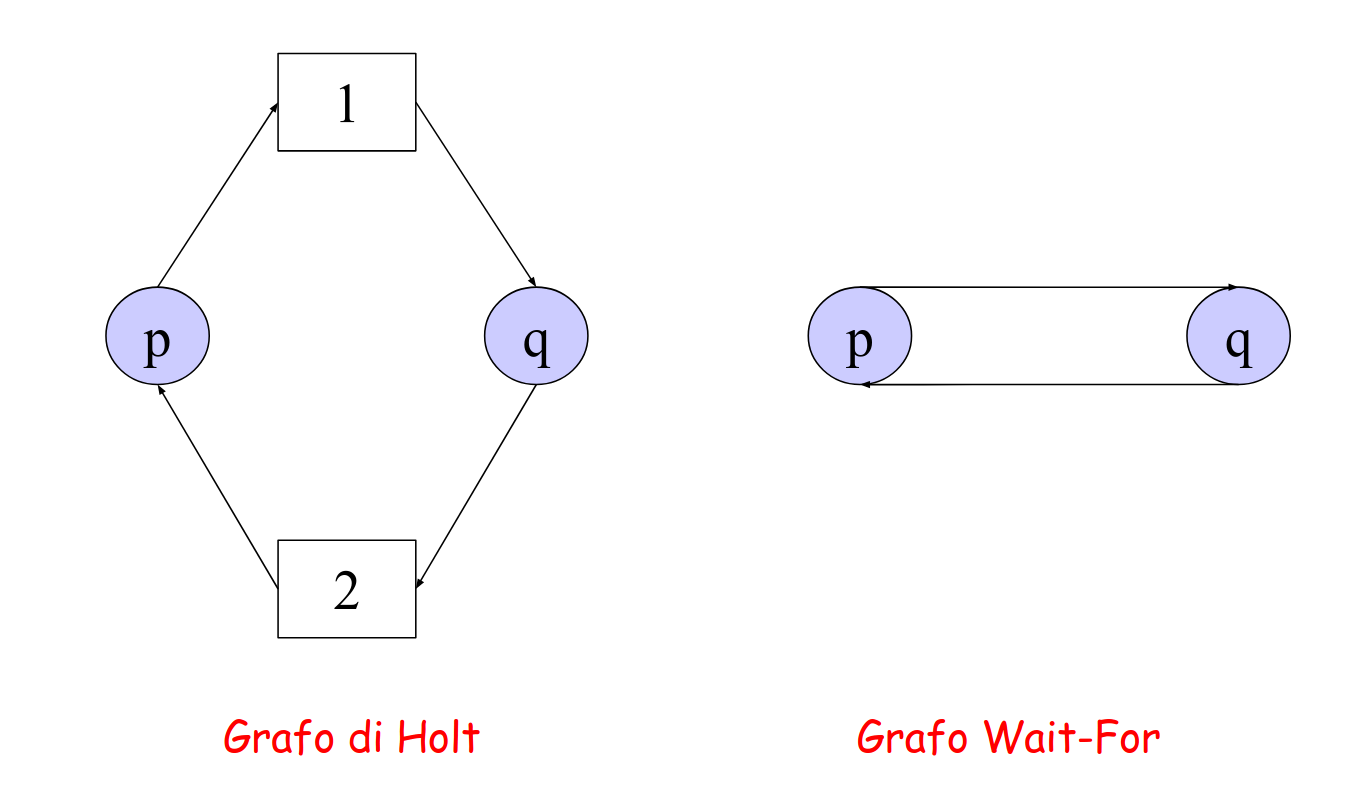
\includegraphics[width=0.4\linewidth]{Images/Screenshot 2024-12-30 at 18-14-14 so-04-risorse - so-04-risorse.pdf.png}
\end{figure}

\subsubsection{Caso 2 - Più risorse per classe}
La presenza di un ciclo nel caso di Holt non è condizione sufficiente per avere deadlock.

\begin{figure} [h]
    \centering
    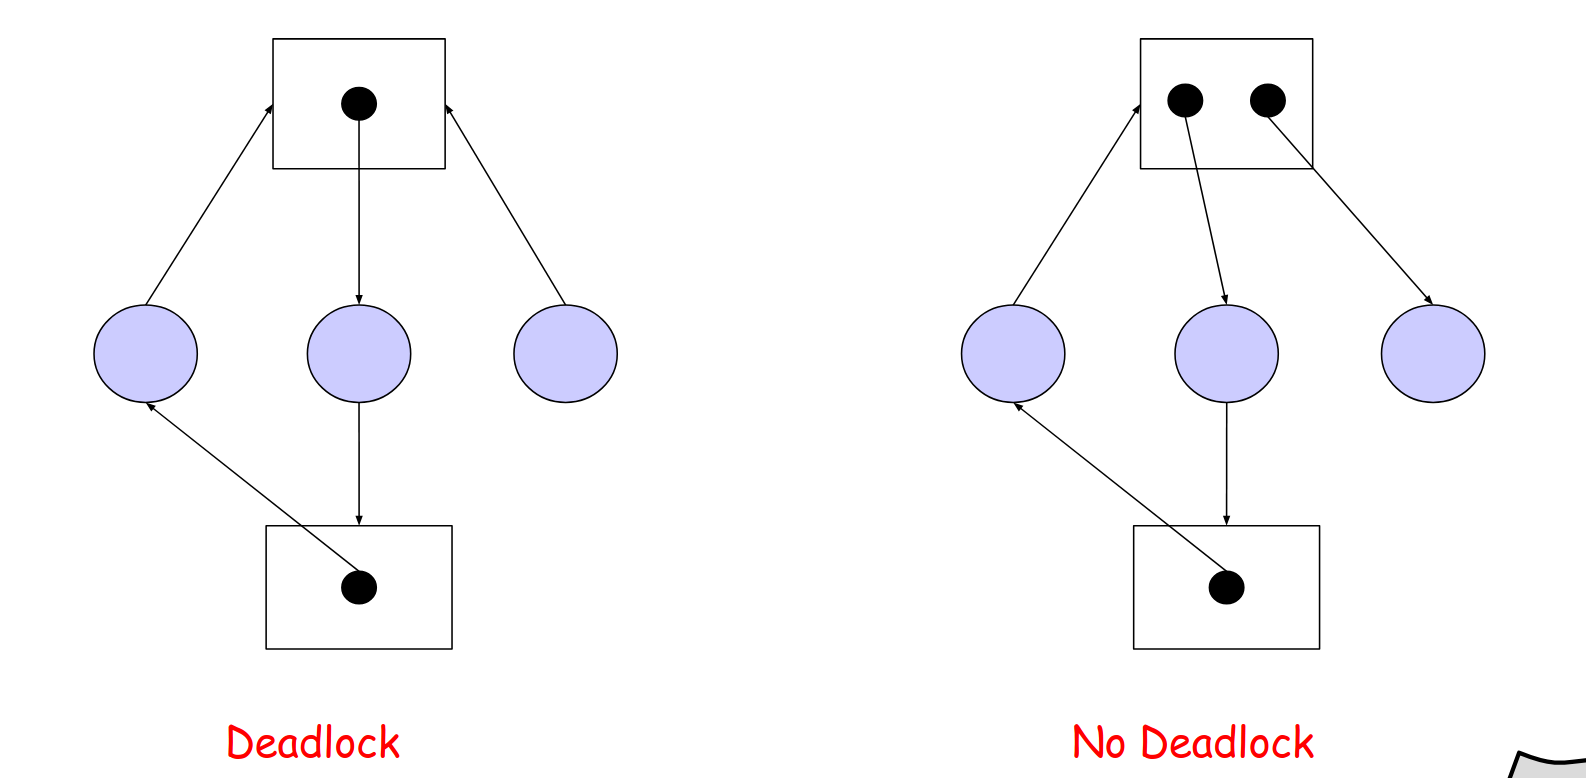
\includegraphics[width=0.5\linewidth]{Images/Screenshot 2024-12-30 at 18-16-02 so-04-risorse - so-04-risorse.pdf.png}
\end{figure}

\subsubsection{Riducibilità di un grafo di Holt}
\paragraph{Definizione:}un grafo di Holt si dice riducibile se esiste almeno un nodo processo con solo archi entranti
\paragraph{Riduzione:} consiste nell'eliminare tutti gli archi di tale nodo e riassegnare le risorse ad altri processi.

\paragraph{Qual è la logica?}eventualmente, un nodo che utilizza una risorsa prima o poi la rilascerà; a quel punto, la risorsa può essere riassegnata.

\begin{figure} [h]
    \centering
    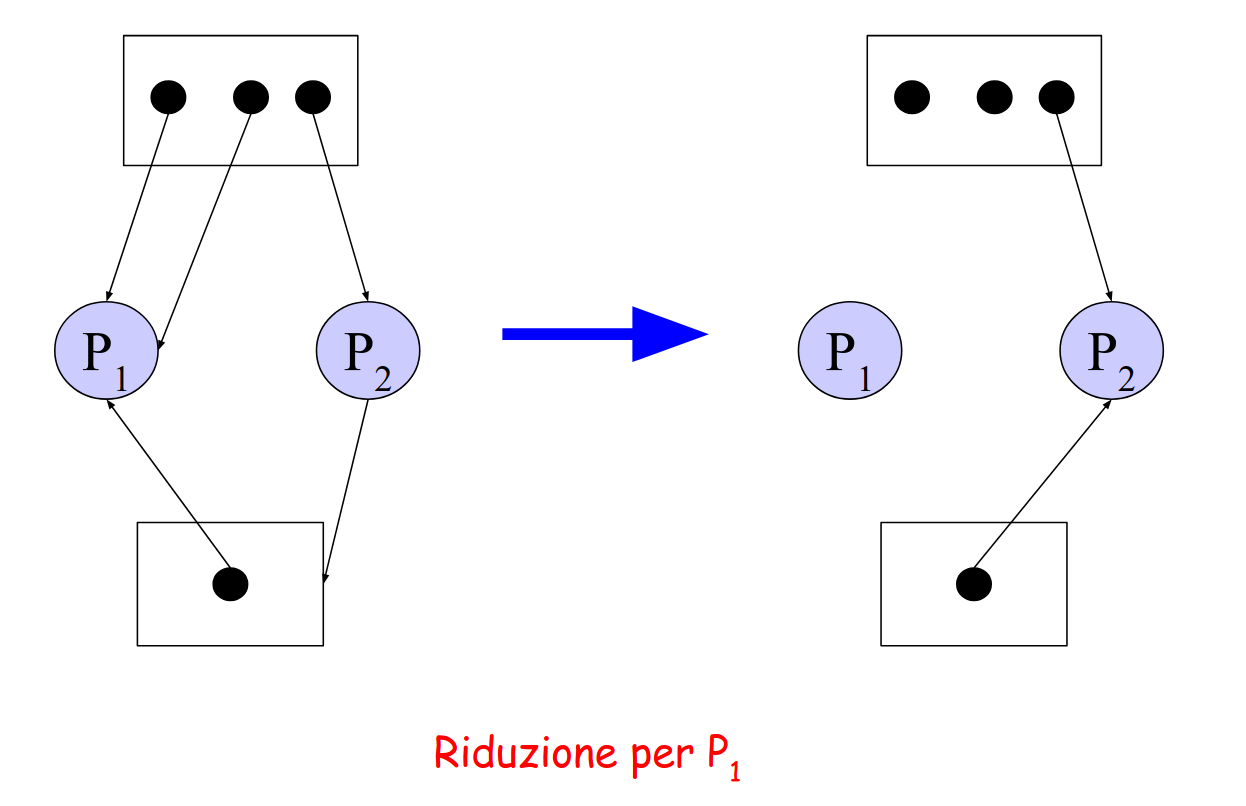
\includegraphics[width=0.5\linewidth]{Images/Screenshot 2024-12-30 at 18-18-35 so-04-risorse - so-04-risorse.pdf.png}
    \caption{Esempio di riduzione}
\end{figure}

\subsubsection{Deadlock detection con grafo di Holt}
\paragraph{Teorema:} se le risorse sono ad accesso mutualmente esclusivo, seriali e non prerilasciabili,  lo stato non è di deadlock se e solo se il grafo di Holt è completamente
riducibile. \textit{(esiste una sequenza di passi di riduzione che elimina tutti gli archi del grafo)}

\subsubsection{Deadlock detection - Knot}

\paragraph{Definizione:} dato un nodo n, l'insieme dei nodi raggiungibili da n viene detto insieme di raggiungibilità di n (scritto \textit{R(n)})

 Un knot del grafo G è il massimo sottoinsieme (non banale) di nodi M tale che per ogni n in M, \textit{R(n)=M}
 
In altre parole: partendo da un qualunque nodo di M, si possono raggiungere tutti i nodi di M e nessun nodo all'infuori di esso.

\begin{figure} [h]
    \centering
    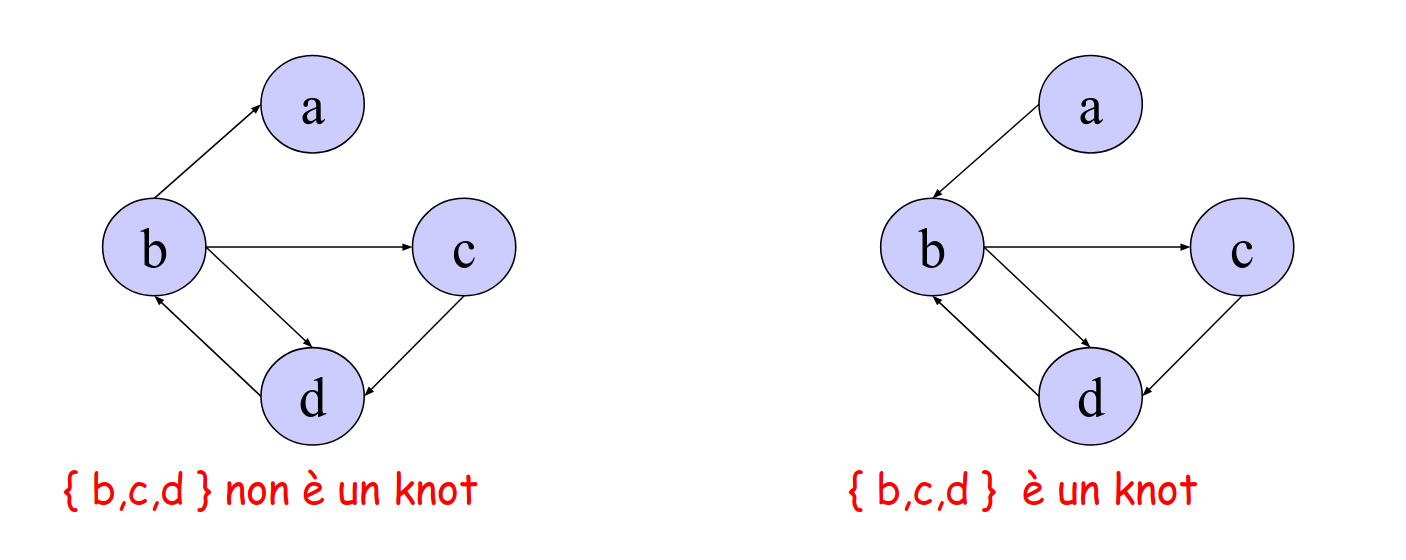
\includegraphics[width=0.6\linewidth]{Images/Screenshot 2025-01-14 at 17-54-33 so-04-risorse - so-04-risorse.pdf.png}
\end{figure}

\paragraph{Teorema:} dato un grafo di Holt con una sola richiesta sospesa per processo
se le risorse sono ad accesso mutualmente esclusivo, seriali e non
prerilasciabili,  allora il grafo rappresenta uno stato di deadlock se e solo se esiste un knot.

\subsection{Deadlock recovery}
Dopo aver rilevato un deadlock bisogna risolvere la situazione.

La soluzione può essere:
\begin{itemize}
    \item \textbf{Manuale:} l'operatore viene informato e eseguirà alcune azioni che permettano al sistema di proseguire.
    \item \textbf{Automatica:} il sistema operativo è dotato di meccanismi che permettono di risolvere in modo automatico la situazione, in base ad alcune politiche
\end{itemize}

\subsubsection{Meccanismi per il deadlock recovery}
\begin{itemize}
    \item Terminazione totale: tutti i processi coinvolti vengono terminati.
    \item Terminazione parziale: viene eliminato un processo alla volta, fino a quando il deadlock non scompare.
    \item Preemption: una risorsa (o più di una, se necessario) viene sottratta ad uno dei processi coinvolti nel deadlock.
    \item Checkpoint/rollback: lo stato dei processi viene periodicamente salvato su disco
(checkpoint). 
In caso di deadlock, si ripristina (rollback) uno o più processi
ad uno stato precedente, fino a quando il deadlock non scompare
\end{itemize}


Terminare processi può essere costoso, questi processi possono essere stati eseguiti per molto tempo; se terminati, dovranno ripartire da capo.
Terminare processi può lasciare le risorse in uno stato inconsistente, se un viene terminato nel mezzo di una sezione critica.

Fare preemption non sempre è possibile, può richiedere interventi manuali.

\subsection{Deadlock prevention e avoidance}
Prevention: per evitare il deadlock si elimina una delle quattro condizioni del deadlock così il deadlock viene eliminato strutturalmente.

Avoidance: prima di assegnare una risorsa ad un processo, si controlla se l'operazione può portare al pericolo di deadlock e in caso, l'operazione viene ritardata.

\subsubsection{Prevention}
Attaccare la condizione di "Mutua esclusione", permettere la condivisione di risorse.

Problemi dello spooling: in generale, lo spooling non sempre è applicabile perchè sposta il problema verso altre risorse.

Attaccare la condizione di "Richiesta bloccante"
\textit{Allocazione totale}, è possibile richiedere che un processo richiede tutte le risorse all'inizio della computazione.
I problemi possono essere: non sempre l'insieme di richieste è noto fin dall'inizio e si riduce il parallelismo.

Attaccare la condizione di "Assenza di prerilascio" non sempre è possibile e può richiedere interventi manuali.

Attaccare la condizione di "Attesa Circolare" \textit{Allocazione gerarchica}, quando alle classi di risorse vengono associati valori di priorità, ogni processo in ogni istante può allocare solamente risorse di priorità superiore a quelle che già possiede.
Se un processo vuole allocare una risorsa a priorità inferiore, deve prima rilasciare tutte le risorse con priorità uguale o superiore a quella desiderata.

L' allocazione gerarchica e allocazione totale danno problemi.
Prevengono il verificarsi di deadlock, ma sono altamente inefficienti perché nell'allocazione gerarchica: l'indisponibilità di una risorsa ad alta priorità ritarda processi che già
detengono risorse ad alta priorità.

Nell'allocazione totale: anche se un processo ha necessità di risorse per poco tempo deve allocarla per tutta la propria esistenza.

\subsubsection{Avoidance - Algoritmo del Banchiere}
Avoidance è l'azione per cui prima di far qualcosa si verifica se porterà a deadlock.

L'algoritmo del banchiere è un algoritmo per evitare lo stallo sviluppato da Dijkstra (1965). 

Il nome deriva dal metodo utilizzato da un ipotetico banchiere di provincia che gestisce un gruppo di clienti a cui ha concesso del credito; non tutti i clienti avranno bisogno dello stesso credito simultaneamente.
\newpage
\section{Algoritmo del Banchiere}
\subsection{Algoritmo del Banchiere Singola valuta}
\paragraph{Descrizione:} 
Un banchiere desidera condividere un capitale (fisso) con un numero
(prefissato) di clienti.

Ogni cliente specifica in anticipo la sua necessità massima di denaro che ovviamente non deve superare il capitale del banchiere.
I clienti fanno due tipi di transazioni: richieste di prestito
e restituzioni.

Il denaro prestato ad ogni cliente non può mai eccedere la necessità massima specificata a priori.

Ogni cliente può fare richieste multiple, fino al massimo importo specificato, una volta che le richieste sono state accolte e il denaro è stato ottenuto deve garantire la restituzione in un tempo finito.

\paragraph{Metodo di funzionamento:} Il banchiere deve essere in ogni istante in grado di soddisfare tutte le richieste dei clienti, o concedendo immediatamente il prestito oppure comunque facendo loro aspettare la disponibilità del denaro in un tempo
finito.

Teniamo conto le seguenti variabili:
\begin{itemize}
    \item $N$ - il numero dei clienti
    \item $IC$ - capitale iniziale
    \item $c_i$ - limite di credito del cliente i ($c_i$ < $IC$)
    \item $p_i$ : denaro prestato al cliente i ($p_i \le c_i$ )
    \item $n_i = c_i - p_i$  - credito residuo del cliente i
    \item $SC$ = $IC - \sum_{i=1}^{N}p_i$ -  saldo di cassa 
\end{itemize}

\paragraph{Stato SAFE}
Le richieste che ogni cliente i può fare possono essere soddisfatte dalle risorse attualmente disponibili più tutte le risorse detenute dai processi j soddisfatti precedentemente ($j < i$).
\paragraph{}
Sia s una permutazione dei valori 1...N. \textit{Esempio, con N=4 e s=(1, 3, 4, 2)}

Indichiamo con s(i) l'i-esima posizione della sequenza.

\subparagraph{Si calcoli il vettore \textbf{avail} come segue:}
\begin{itemize}
    \item $avail[1] = SC$
    \item $avail[j+1] = avail[j] + p_{s(j)}$ , con j=1...N-1
\end{itemize}

Uno stato del sistema si dice safe se vale la seguente condizione:
$n_{s(j)} \le avail[j]$ , con j=1...N

\paragraph{Lo stato UNSAFE} è condizione necessaria ma non sufficiente per non avere deadlock. Un sistema in uno stato UNSAFE può evolvere senza procurare alcun deadlock.

\subsubsection{Esempio - stato SAFE} 

\begin{figure}[h]
    \centering
    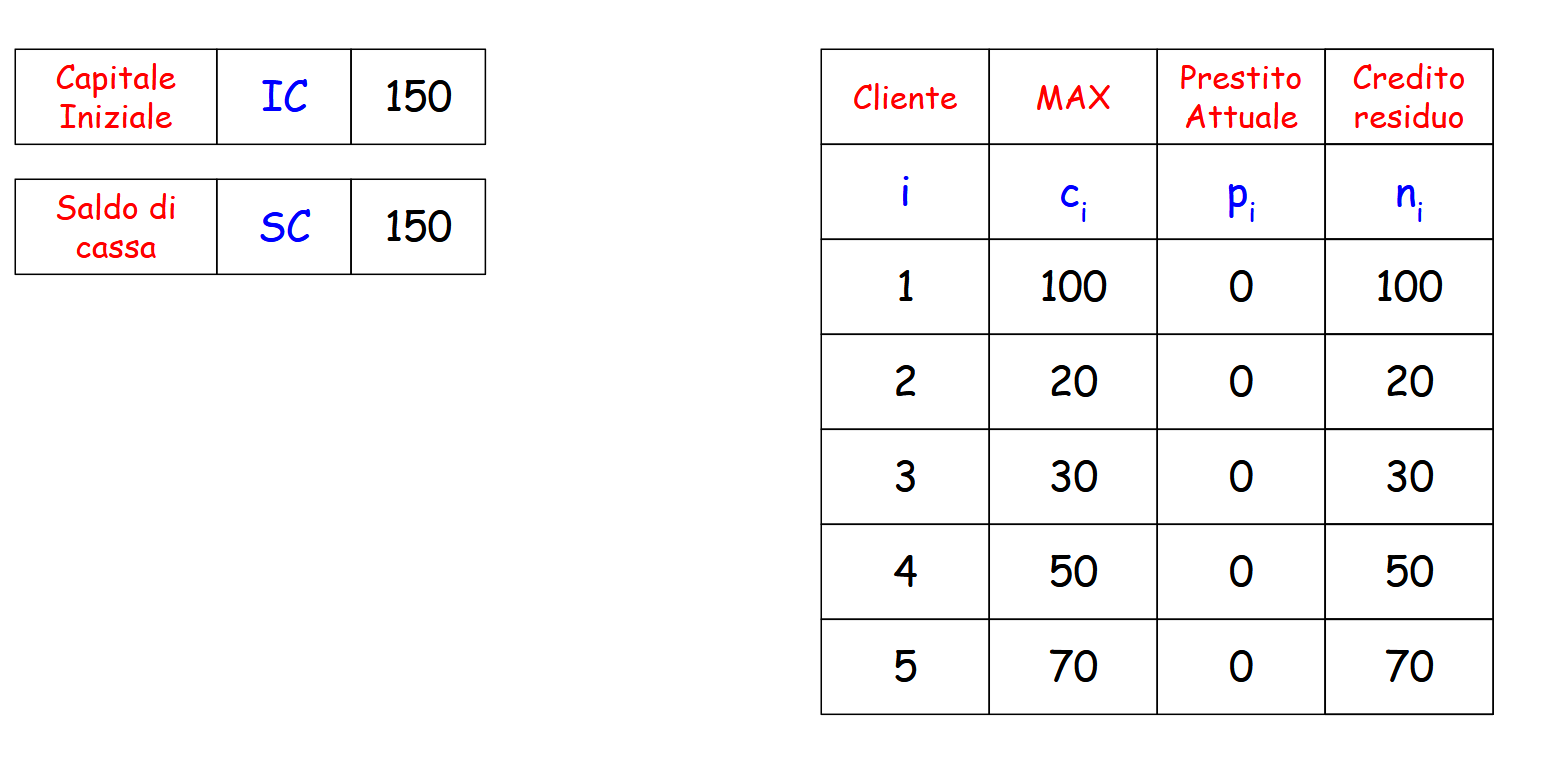
\includegraphics[width=0.7\linewidth]{Images/Screenshot 2025-01-15 113351.png}
    \caption{Situazione iniziale}
\end{figure}

Regola pratica (per il banchiere a singola valuta):
lo stato SAFE può essere verificato usando la sequenza che ordina in modo crescente i valori di $n_i$ (credito residuo di i).

Sono sicuro che concedo ad ogni passo il minimo possibile per poi recuperarlo e aumentare la disponibilità di prestito per il prossimo cliente.
\newpage 

\begin{figure} [h]
    \centering
    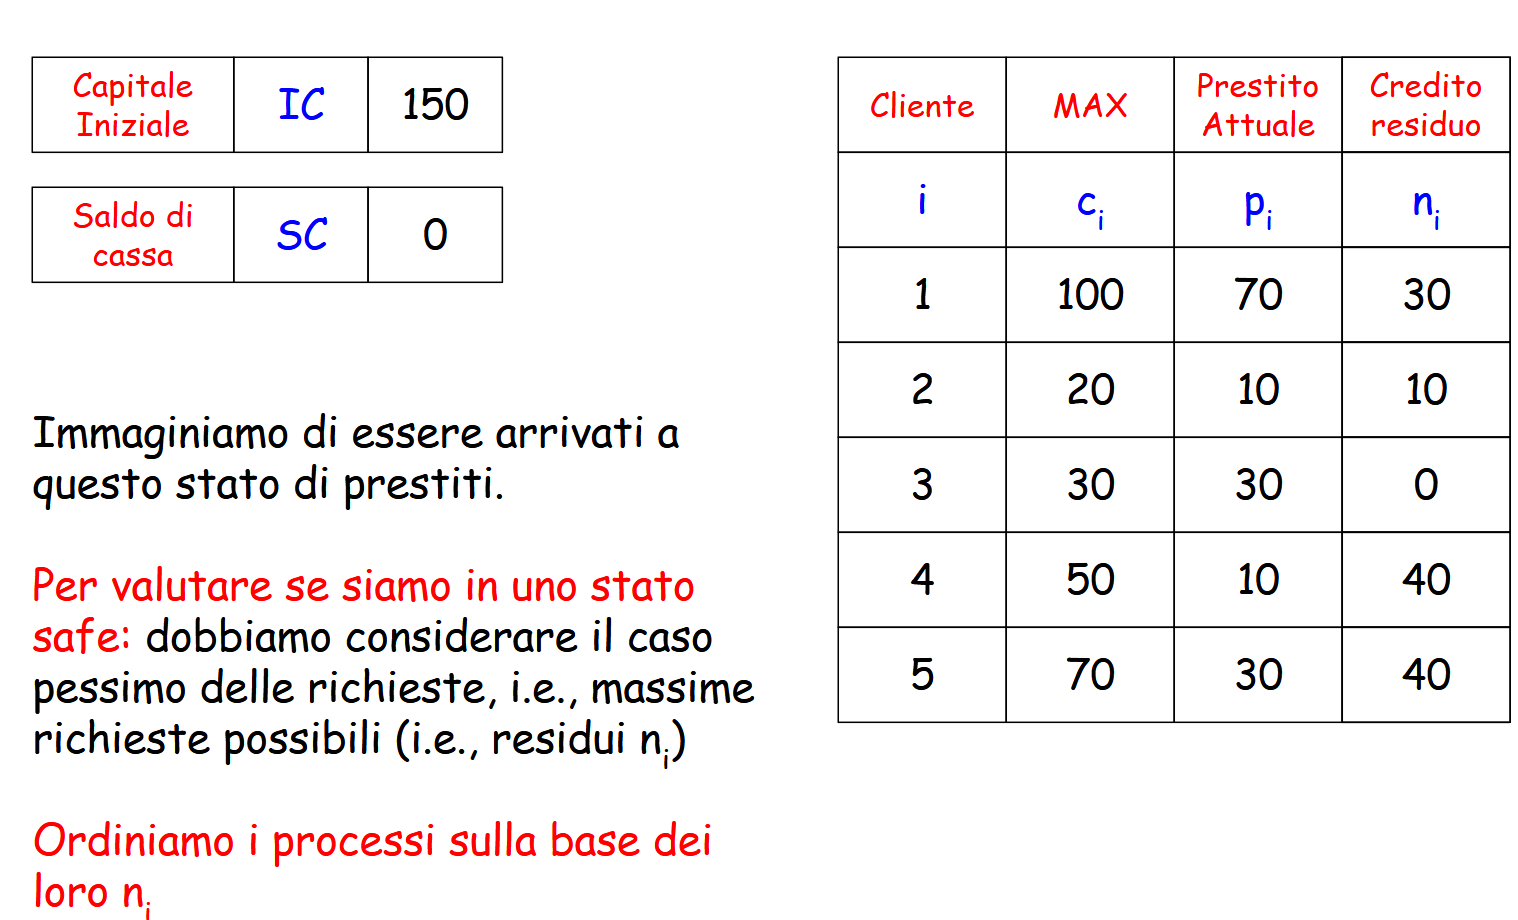
\includegraphics[width=0.7\linewidth]{Images/Screenshot 2025-01-15 113840.png}
\end{figure}

\begin{figure} [h]
    \centering
    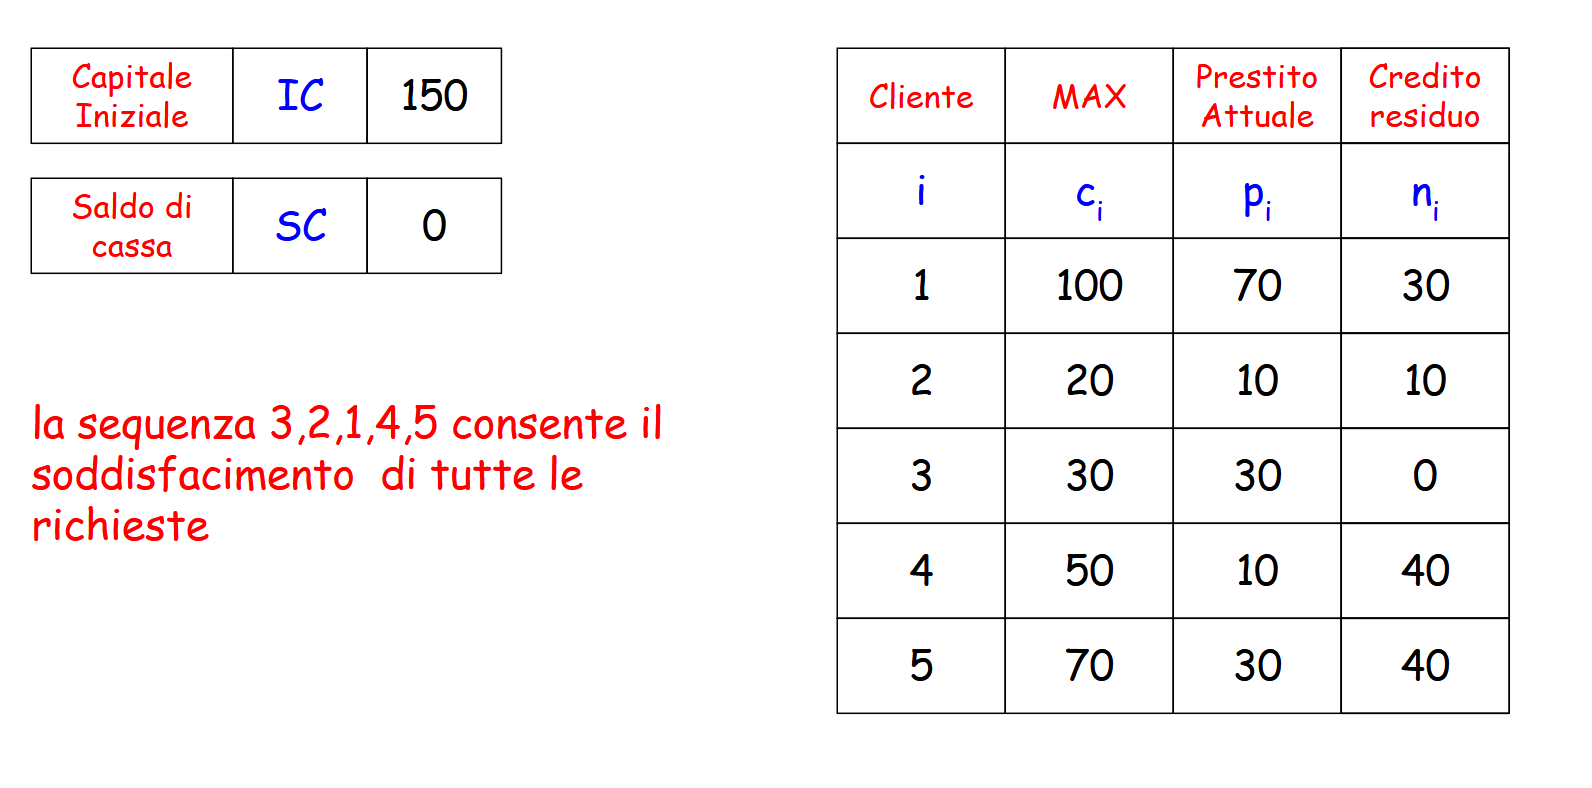
\includegraphics[width=0.7\linewidth]{Images/Screenshot 2025-01-15 114120.png}
\end{figure}

\begin{figure} [h]
    \centering
    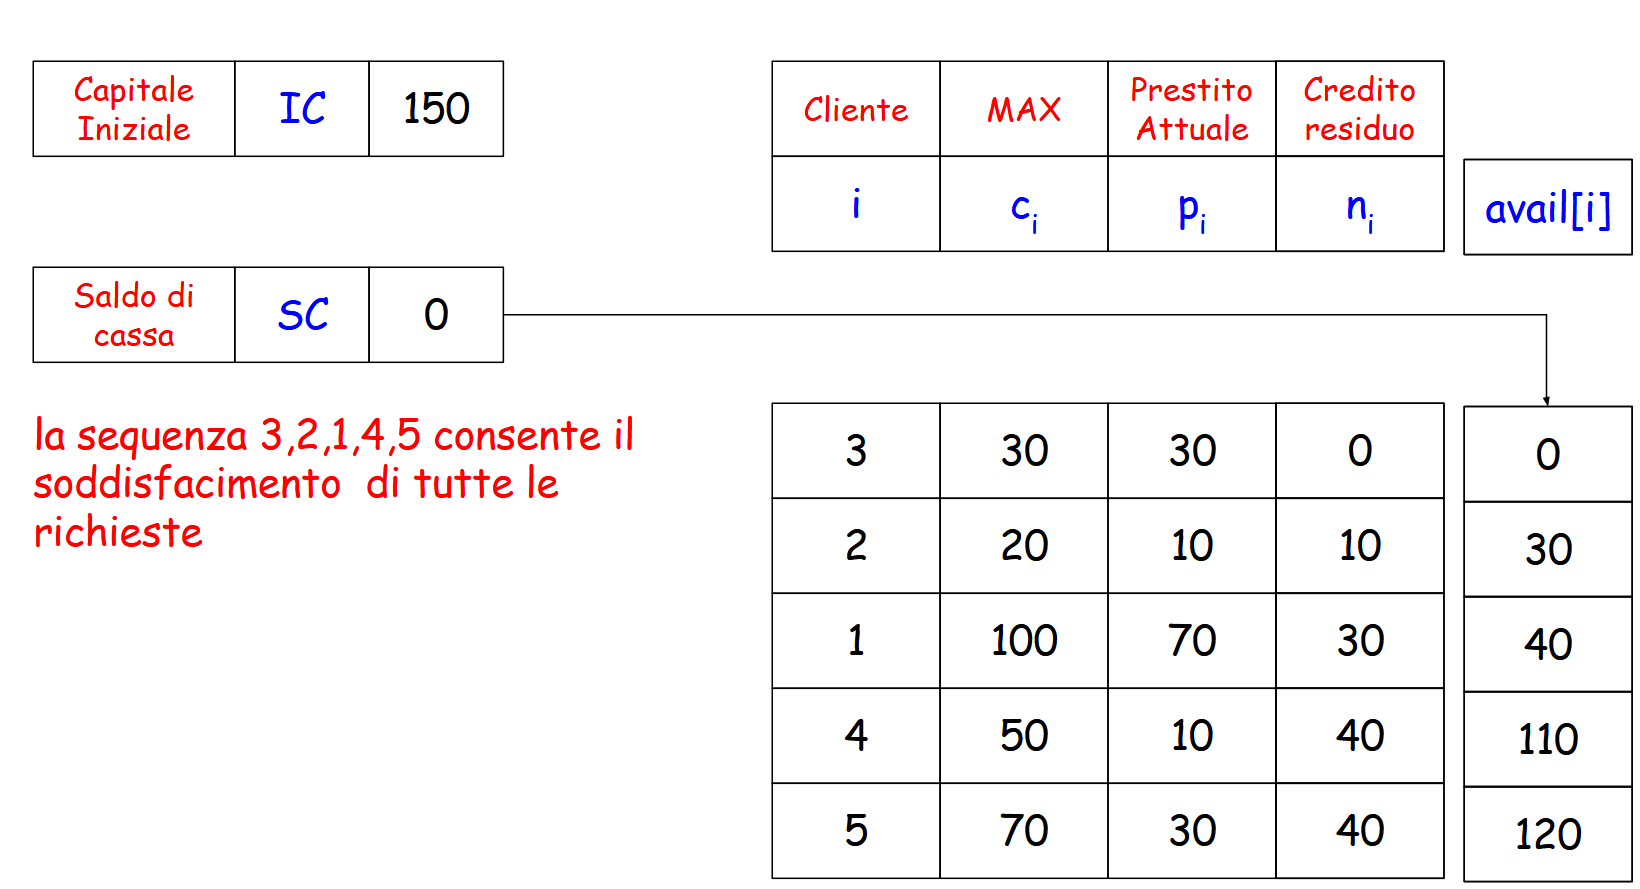
\includegraphics[width=0.7\linewidth]{Images/Screenshot 2025-01-15 114202.png}
\end{figure}

\newpage

\subsubsection{Esempio - stato UNSAFE} 

\begin{figure} [h]
    \centering
    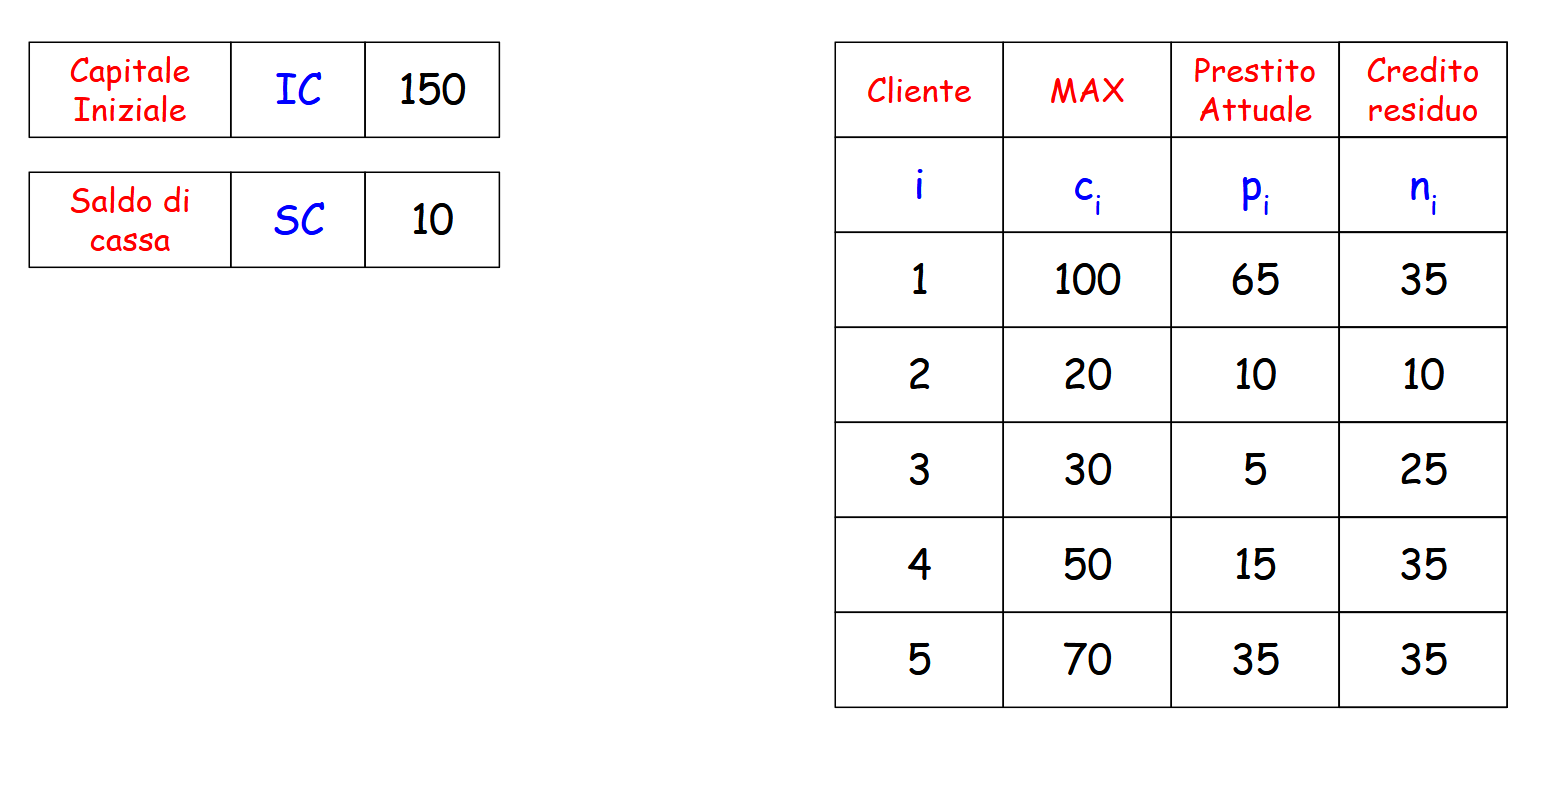
\includegraphics[width=0.7\linewidth]{Images/Screenshot 2025-01-15 114320.png}
\end{figure}

\begin{figure} [h]
    \centering
    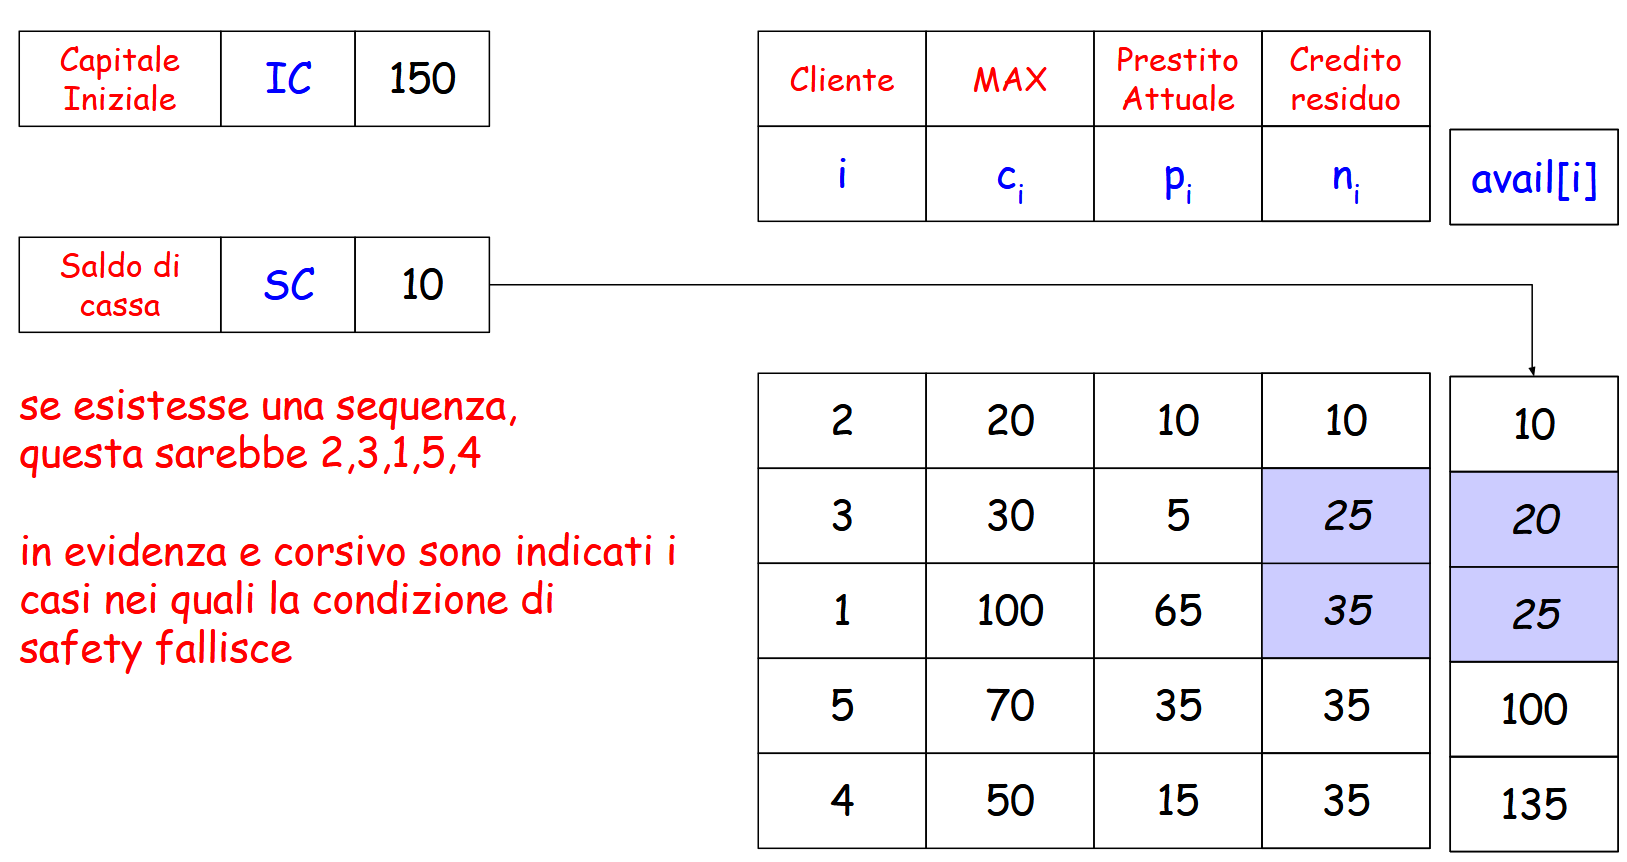
\includegraphics[width=0.7\linewidth]{Images/Screenshot 2025-01-15 114534.png}
\end{figure}

\begin{figure} [h]
    \centering
    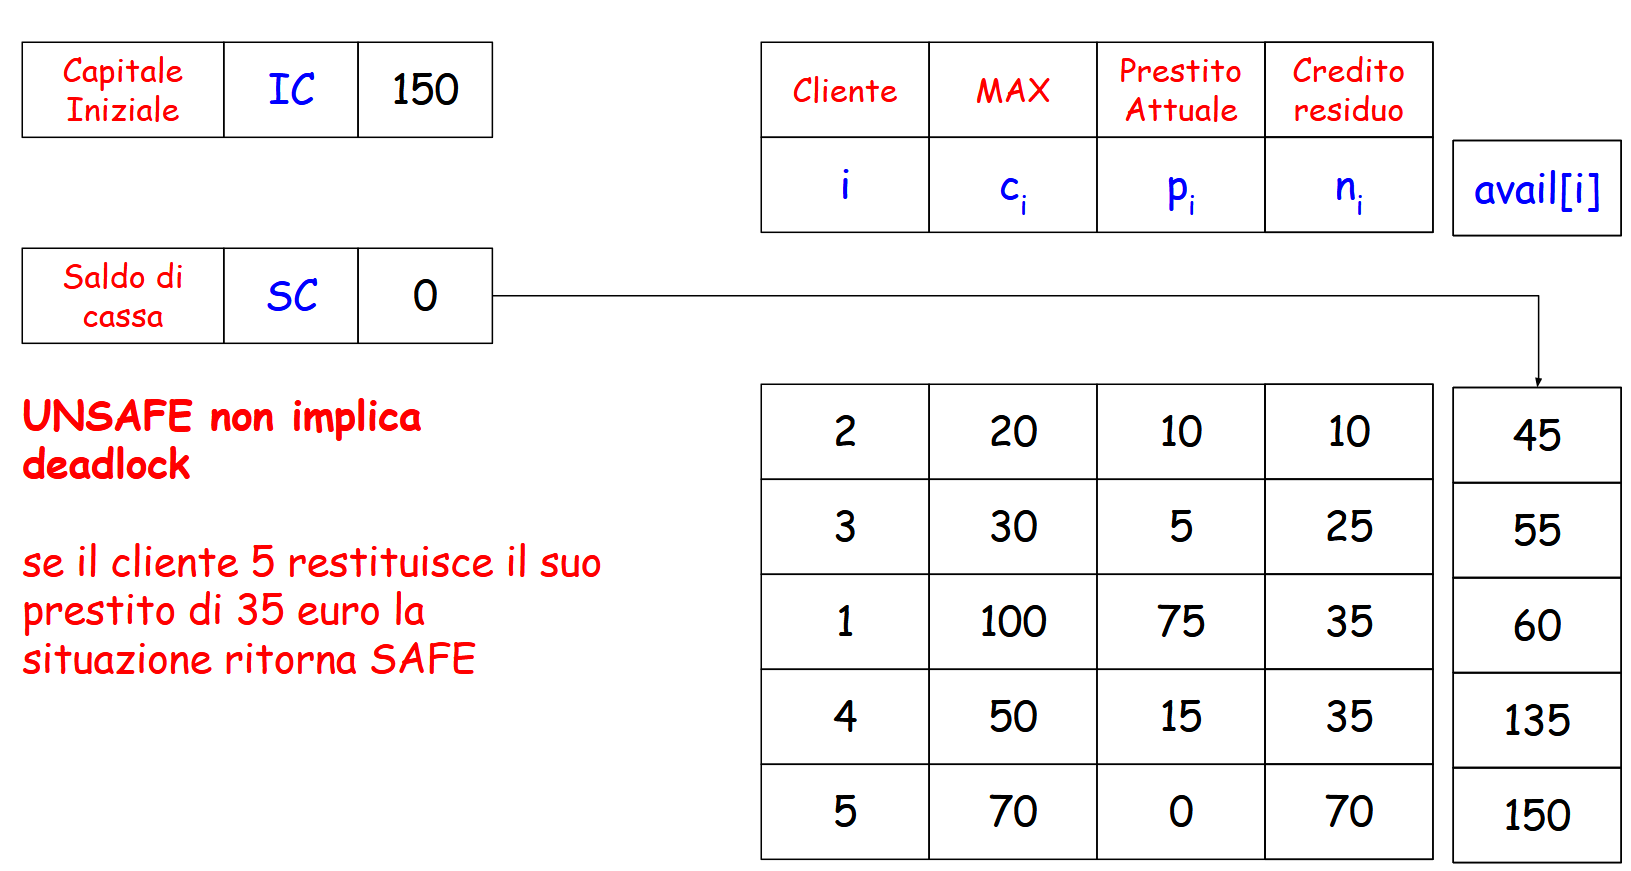
\includegraphics[width=0.7\linewidth]{Images/Screenshot 2025-01-15 114907.png}
\end{figure}

\subsubsection{Conclusione Algoritmo Banchiere singola valuta}
La similitudine fra banchieri e sistemi operativi ora è chiara: il denaro sono le risorse, il sistema le deve allocare ai processi senza che si possa verificare deadlock.

Le definizioni viste fino a questo punto riguardano il caso teorico elementare di un sistema avente un'unica classe di risorse.
\newpage
\subsection{Algoritmo del Banchiere Multivaluta}
L'estensione del problema del banchiere singola valuta dove si ipotizza che il banchiere debba fare prestiti usando valute diverse (euro, dollari, yen, etc.)
Le diverse valute rappresentano diverse classi di risorse.

Teniamo conto le seguenti variabili:
\begin{itemize}
    \item $N$ - il numero dei clienti
    \item $IC_k$ - capitale iniziale della valuta k
    \item $c_{i,k}$ - limite di credito in valuta k del cliente i ($c_{i,k} < IC_k$)
    \item $p_{i,k}$ - denaro prestato in valuta k al cliente i ($p_i,k \le c_{i,k}$)
    \item $n_{i,k} =c_{i,k} - p_{i,k}$ - credito residuo in valuta k del cliente i
    \item $SC_k = IC - \sum_{i=1}^{N} p_{i,k}$ - saldo di cassa in valuta k 
\end{itemize}

\paragraph{Stato SAFE}

Sia s una permutazione dei valori 1...N. Esempio, con N=4 e s=(1, 3, 4, 2).
Indichiamo con s(i) l'i-esima posizione della sequenza.
\subparagraph{Si calcoli il vettore $avail_k$ come segue:}
\begin{itemize}
    \item $avail_k[1] = SC_k$
    \item $avail_k[j+1] = avail_k[j] + p_{s(j)}$ , con j=1...N-1
\end{itemize}

Uno stato del sistema si dice safe se vale la seguente condizione: $n_{s(j),k} \le avail_k[j]$ , con j=1...N

\paragraph{Problema} La regola di ordinare i processi secondo i valori di n i non è applicabile, l'ordine può essere in generale diverso fra le diverse valute gestite dal banchiere.
\paragraph{Soluzione}Si può creare la sequenza procedendo passo passo aggiungendo un processo a caso fra quelli completamente soddisfacibili. Ovvero, al passo j si sceglie quelli per cui: $n_{s(j),k} \le avail_k[j]$

\subsubsection{Esempio - Banchiere Multivaluta}

\begin{figure} [h]
    \centering
    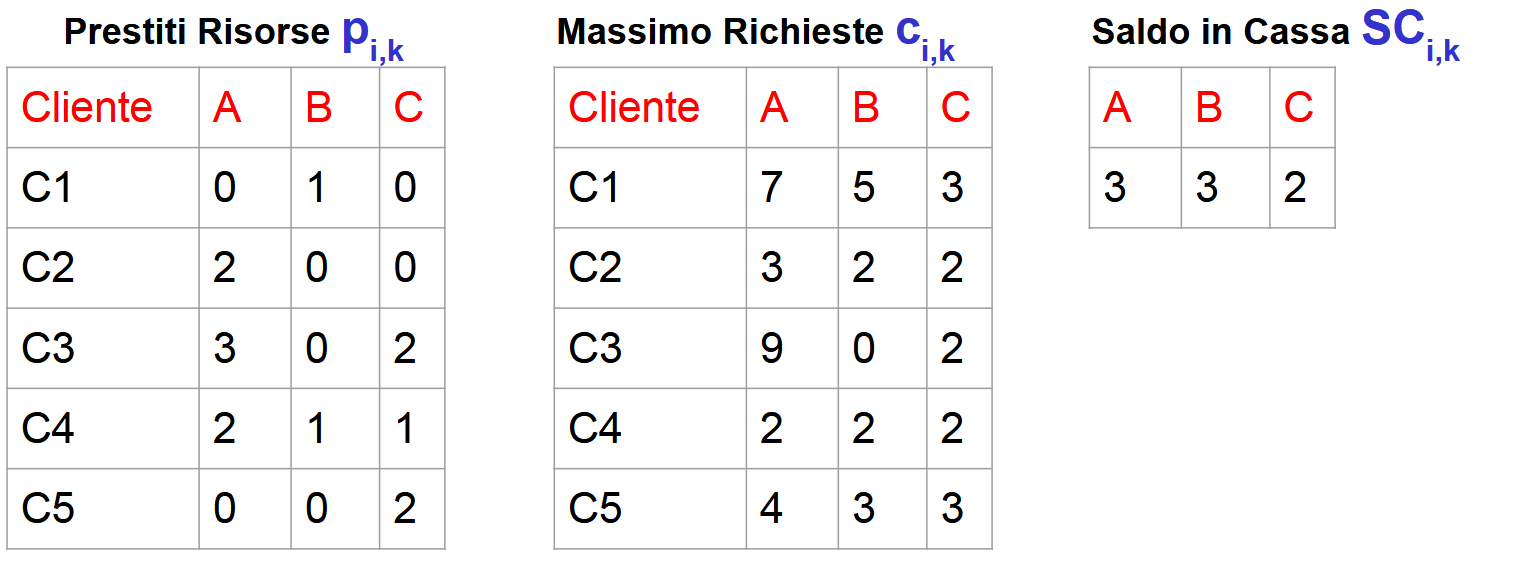
\includegraphics[width=0.65\linewidth]{Images/Screenshot 2025-01-15 122610.png}
\end{figure}

\begin{figure} [h]
    \centering
    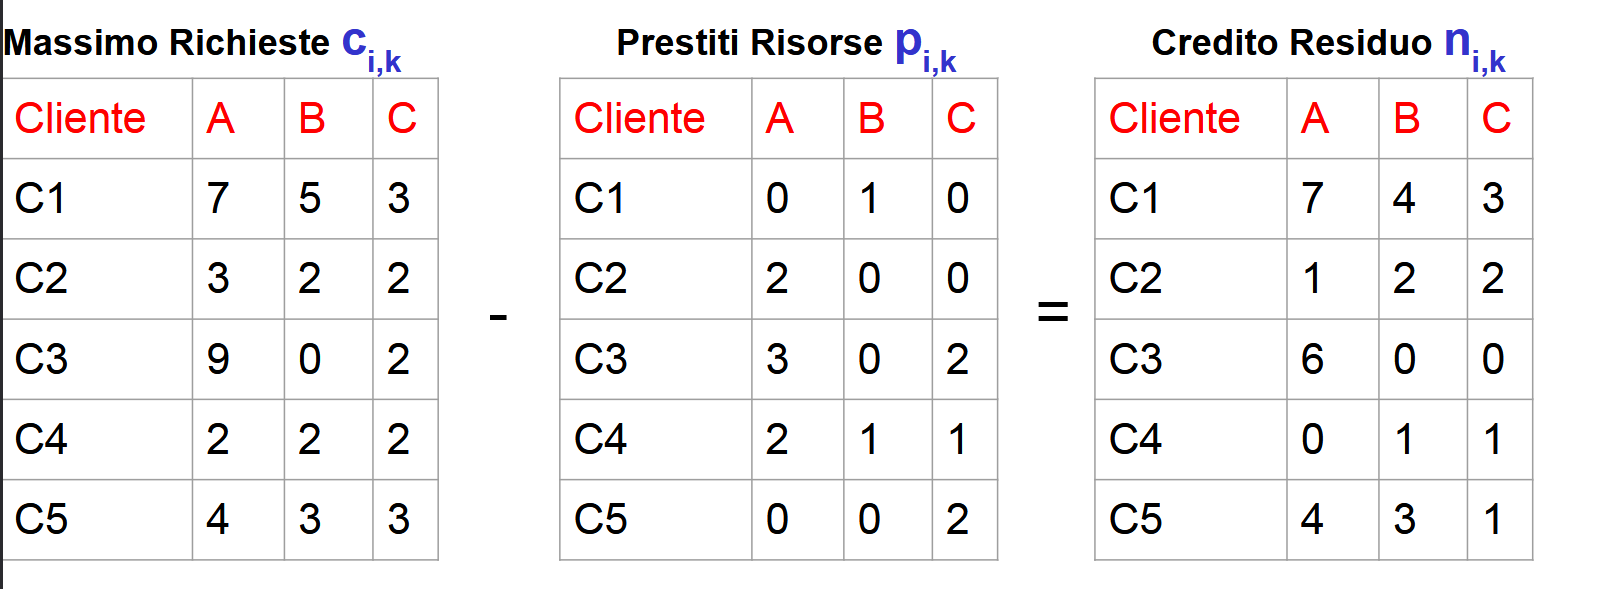
\includegraphics[width=0.65\linewidth]{Images/Screenshot 2025-01-15 122705.png}
\end{figure}

\begin{figure} [h]
    \centering
    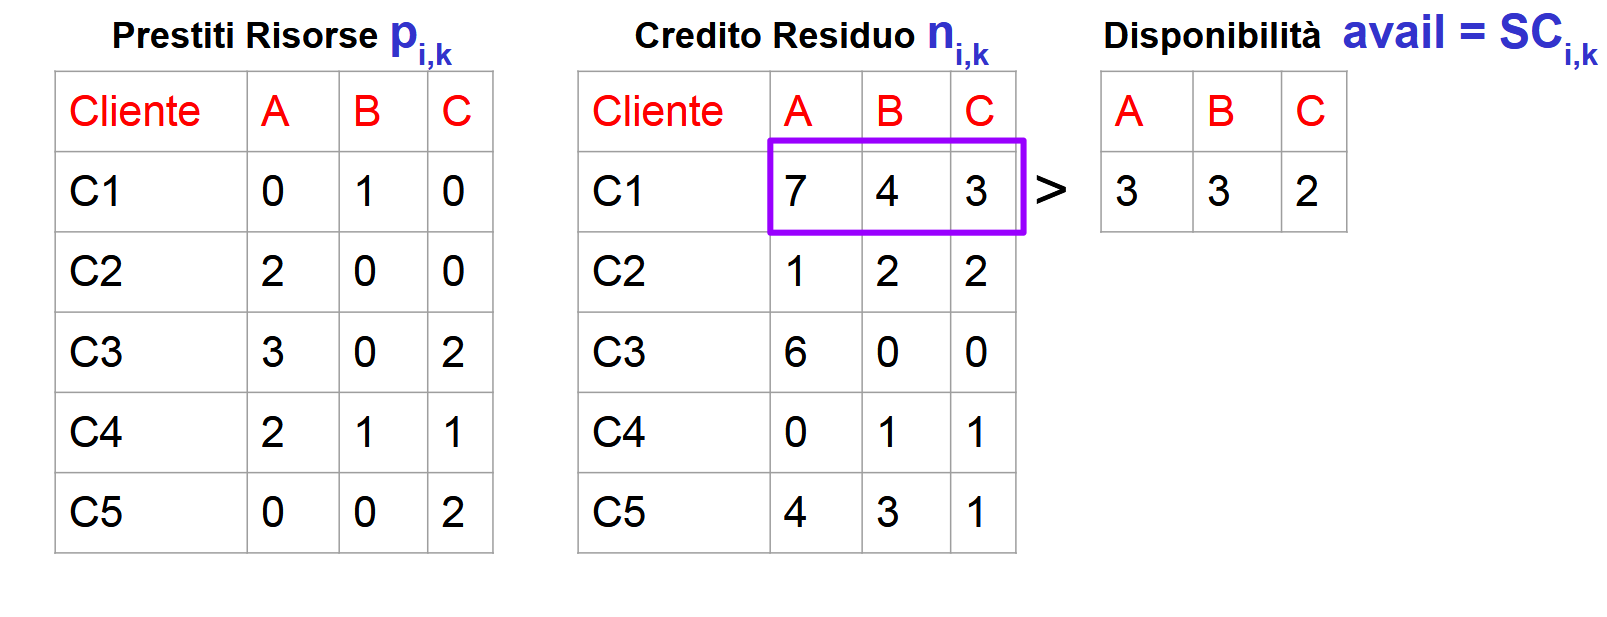
\includegraphics[width=0.65\linewidth]{Images/Screenshot 2025-01-15 122853.png}
\end{figure}

\begin{figure} [h]
    \centering
    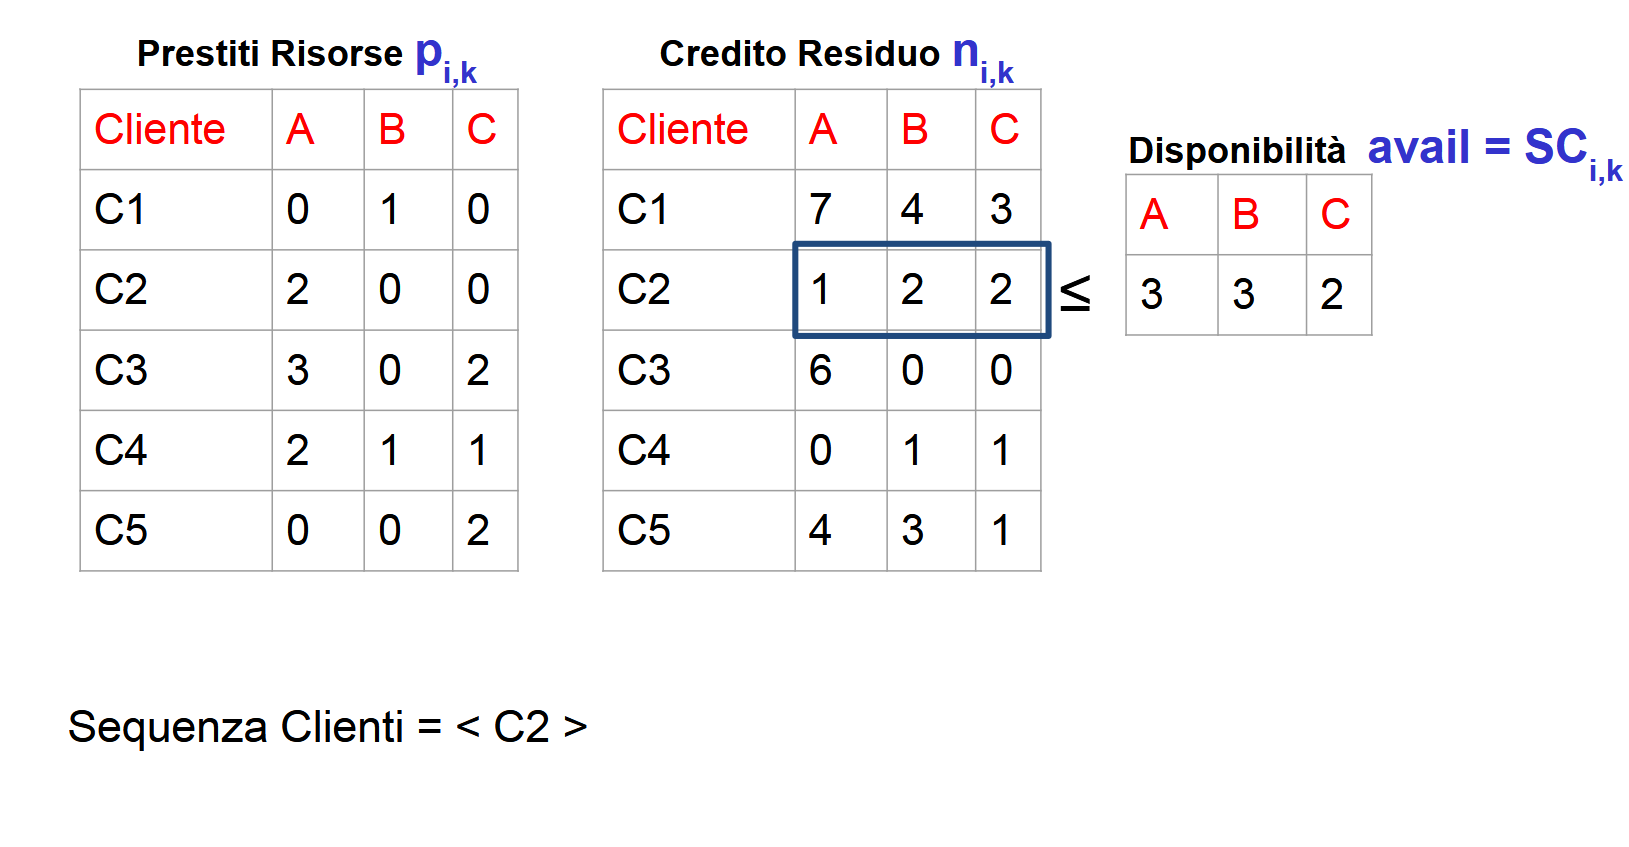
\includegraphics[width=0.65\linewidth]{Images/Screenshot 2025-01-15 123110.png}
\end{figure}

\begin{figure} [h]
    \centering
    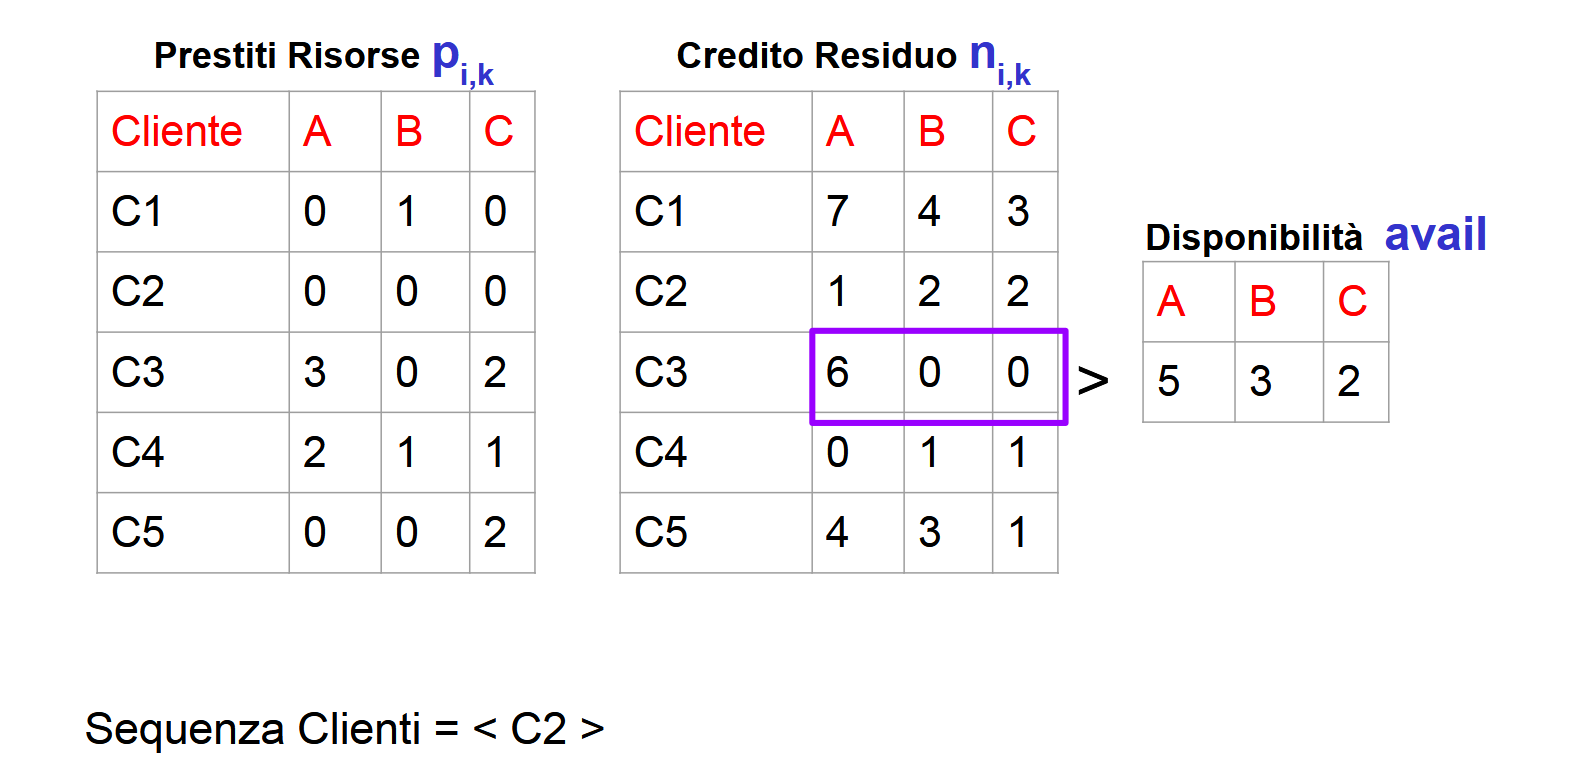
\includegraphics[width=0.65\linewidth]{Images/Screenshot 2025-01-15 125005.png}
\end{figure}

\begin{figure} [h]
    \centering
    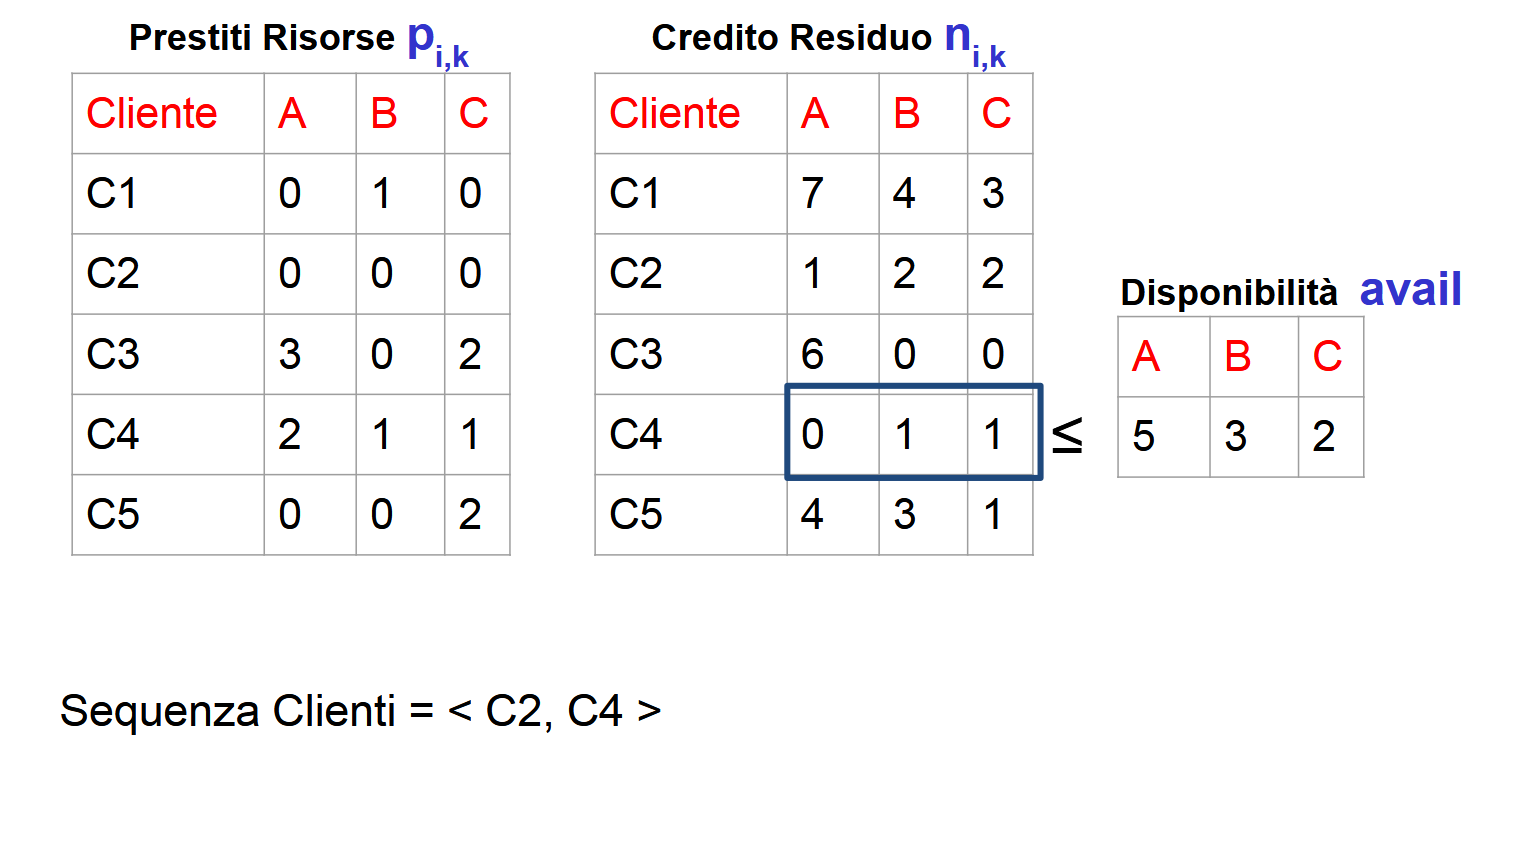
\includegraphics[width=0.65\linewidth]{Images/Screenshot 2025-01-15 125124.png}
\end{figure}

\begin{figure} [h]
    \centering
    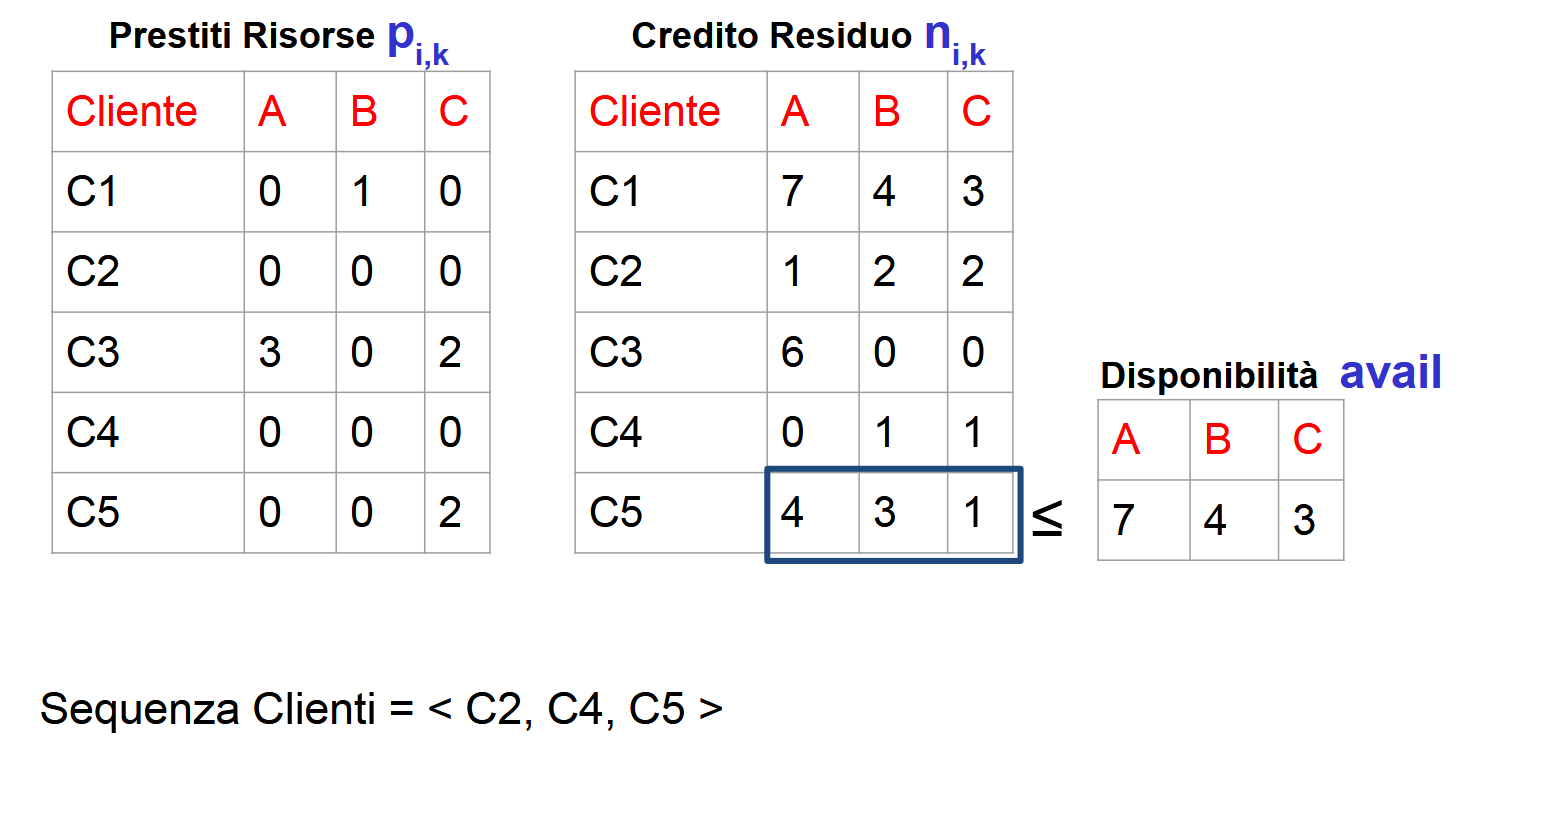
\includegraphics[width=0.65\linewidth]{Images/Screenshot 2025-01-15 125217.png}
\end{figure}

\begin{figure} [h]
    \centering
    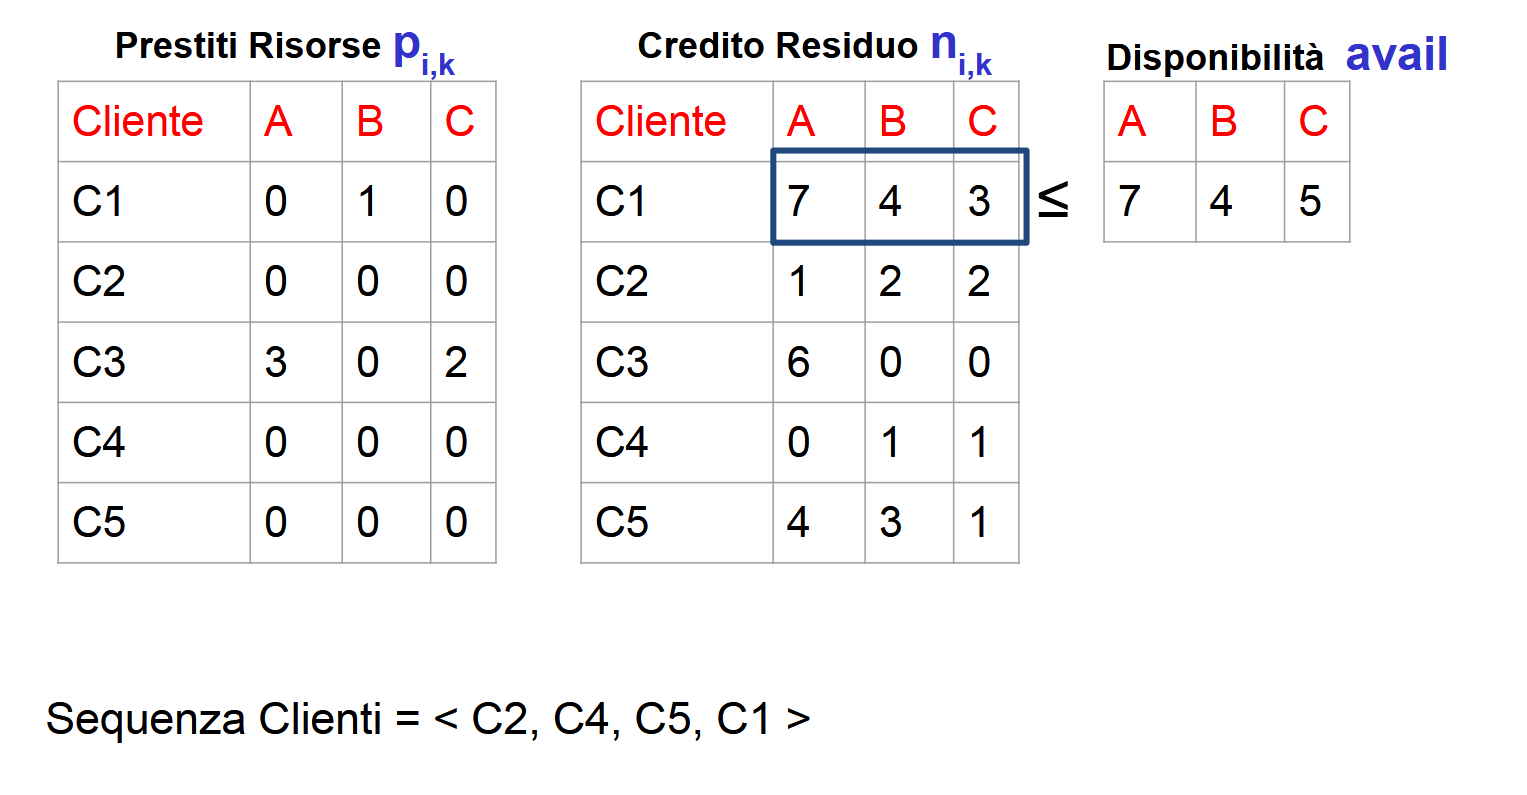
\includegraphics[width=0.65\linewidth]{Images/Screenshot 2025-01-15 125252.png}
\end{figure}

\begin{figure} [h]
    \centering
    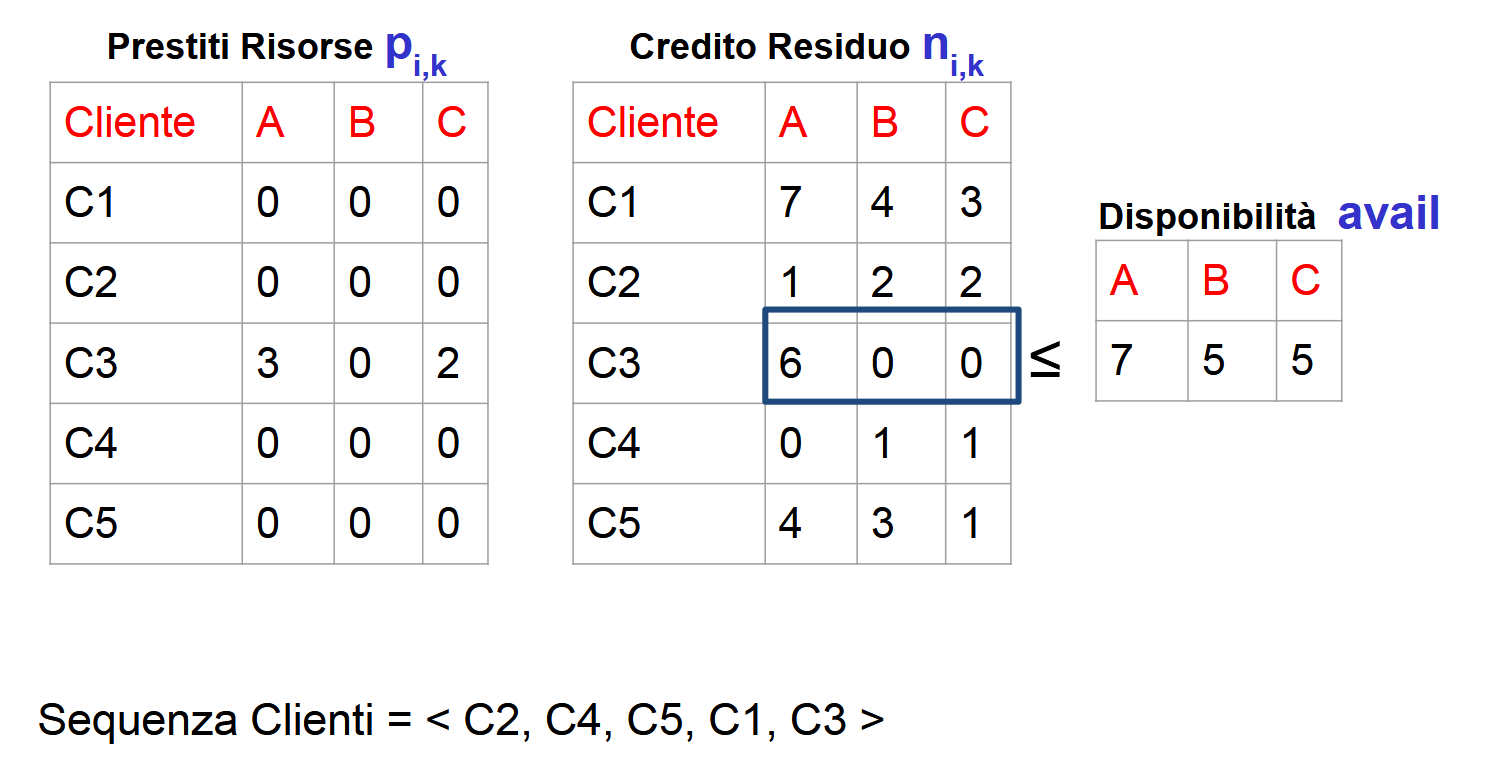
\includegraphics[width=0.65\linewidth]{Images/Screenshot 2025-01-15 125344.png}
\end{figure}

\begin{figure} [h]
    \centering
    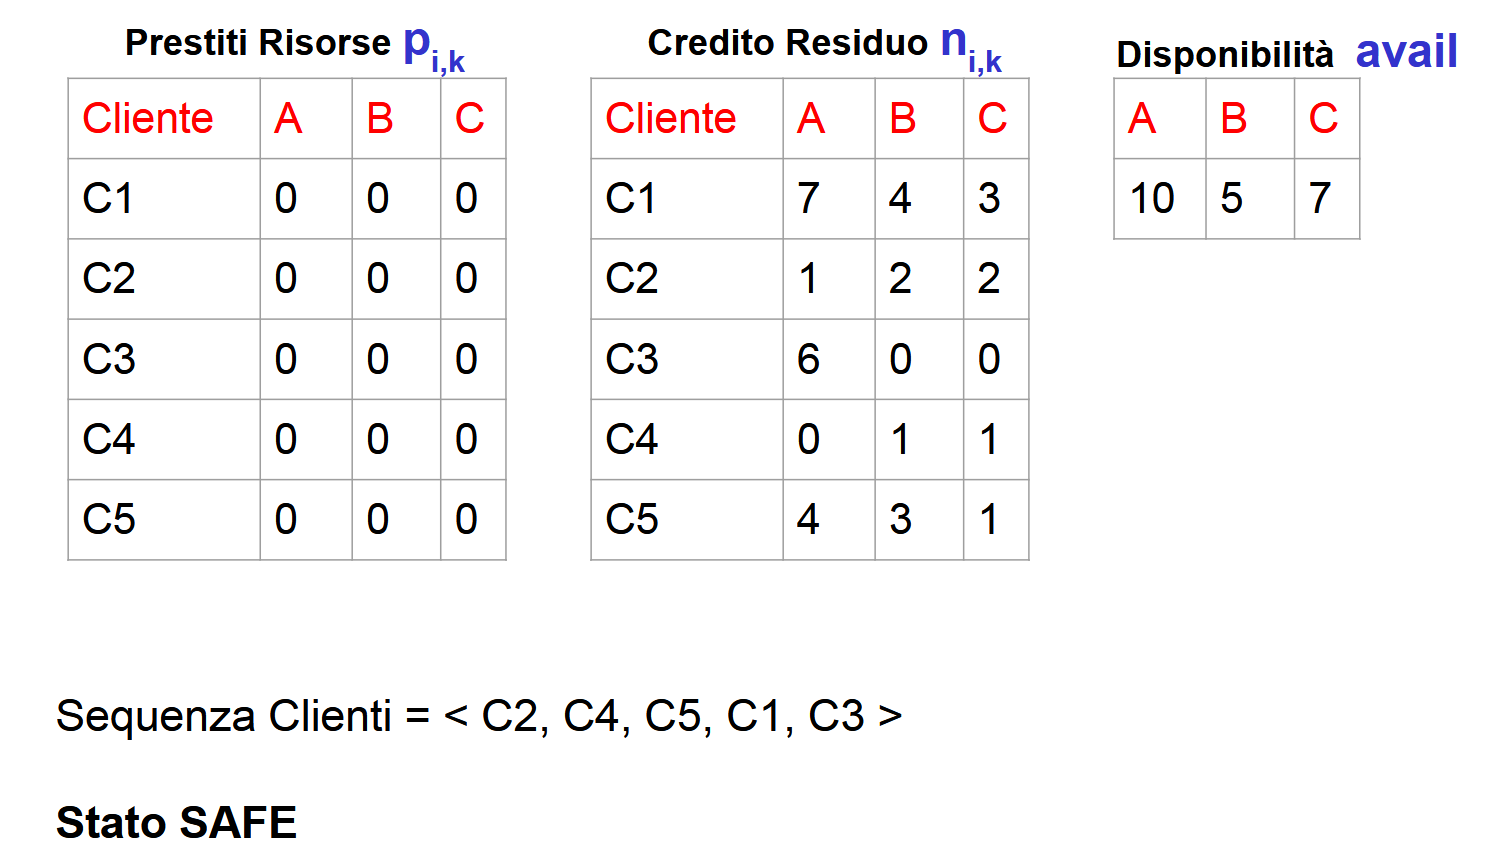
\includegraphics[width=0.65\linewidth]{Images/Screenshot 2025-01-15 125412.png}
\end{figure}
